\chapter{\label{ch:ml}Neural Networks} 

%%%%%%%%%%%%%%%%%%%%%%%%%%%%%%%%%%%%%%%%%%%%%%%%%%%%%%%%%%%%%%%%%%%%%%%%%%%%%%%%
% Relevant bits
%
%   - Neural Network
%   - CNN
%   - Recurrent NN
%   - Backpropagation
%   - Dropout
%   - Inception
%   - Batch normalisation
%
%   - Losses
%     - IOU
%     - 
%
%   - Activations
%     - RELU
%     - Sigmoid
%
%   - Architectures
%%%%%%%%%%%%%%%%%%%%%%%%%%%%%%%%%%%%%%%%%%%%%%%%%%%%%%%%%%%%%%%%%%%%%%%%%%%%%%%%

\minitoc

Machine Learning (ML) is a field of research which studies algorithms which 
can learn to make predictions from data, i.e. predict a set of output variables,
given a set of input variables. The algorithms typically take the form of a
multivariate function, which is used to predict the output \cite{Reed1999}.

ML algorithms are often classified into four groups based on two distinctions: 
regression or classification, and supervised or unsupervised. The first
distinction is based on the nature of the output distribution expected from the
network; regression algorithms are designed to predict the outputs of a 
continuous function, whereas classification algorithms aim to separate data 
into groups. The distinction between supervised and unsupervised algorithms is 
based on the outputs used during training; in a supervised algorithm the true 
output is known, and the network's goal is to predict the true output, while 
in an unsupervised algorithm the output is unknown, and the networks goal is 
to extract meaningful structure from the data.

Chapters \ref{ch:chargeid} and \ref{ch:michel} of this thesis describe two 
examples of the application of Neural Networks (NN) for event reconstruction 
in LArTPC data. These algorithms are classification algorithms based on the
supervised learning approach. This chapter will not provide a full survey of
the available ML techniques, instead it will briefly describe the theory 
behind NNs, as well as providing details of the techniques used in the 
subsequent chapters. 

\section{Artificial Neural Networks}
Artificial neural networks (ANN) are a class of ML algorithm that draw
inspiration from biological neurons. An ANN consists of a set of nodes, along
with a set of connections between those nodes. The set of nodes and connections
is often referred to as a graph or architecture. The nodes in 
the graph take the form of artificial neurons, which pass a number of inputs 
through an activation function to produce a single output, as depicted in 
Figure \ref{fig:neuron}.  The output of each neuron is either distributed to 
subsequent neurons in the network, or it is part of the output of the network. 
\begin{figure}

	\centering

	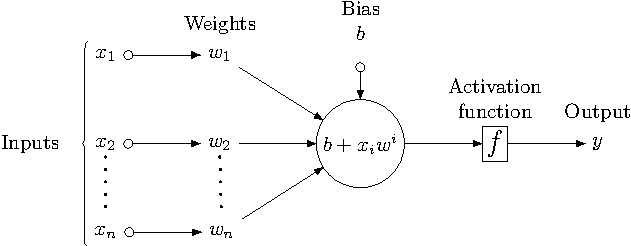
\includegraphics[width = 0.7\textwidth]{figures/neuron.pdf}

	\caption
	[Graphical representation of an individual neuron in an artificial neural
	network.]
	{Graphical representation of an individual neuron in an artificial neural
	network.}

	\label{fig:neuron}

\end{figure}

One of the most widely used ANNs is the multi--layer perceptron 
(MLP)\cite{Reed1999}; this class of network consists of at least three layers 
of nodes: an input layer, one or more hidden layers, and an output layer. The 
layers are connected in a feedforward configuration, such that the graph of 
nodes contains no cycles. The layers of an MLP are often fully connected or 
dense, meaning that the output of every node is connected to the input of 
every node in the next layer of the network. An example of a fully connected 
MLP, with two hidden layers, is shown in Figure \ref{fig:mlp}. 

\begin{figure}

	\centering

	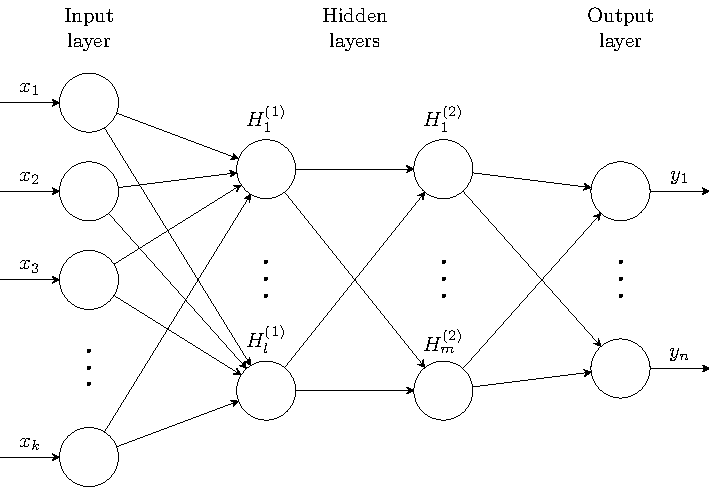
\includegraphics[width = 0.8\textwidth]{figures/mlp.pdf}

	\caption
	[A graphical representation of a multi--layer perceptron.]
	{ A graphical representation of a multi--layer perceptron. }

	\label{fig:mlp}

\end{figure}

Each node receives input from nodes in the previous layer, and uses the inputs
to calculate a response function. For the $i^{th}$ node in the $j^{th}$ layer 
of a network, 
\begin{equation*}
	z^{i,j} = \mathbf{w}^{i,j} \cdot \mathbf{x}^{j-1} + b^{i,j}
\end{equation*}
where $z^{i,j}$ is the response function, $\mathbf{w}^{i,j}$ is the weights
vector, $b^{i,j}$ is the bias, and $\mathbf{x}^{j-1}$ is the input vector from 
the previous layer. This response function is usually passed through a
nonlinear activation function, $f$, to produce the output from the node,
$y$, which is part of the input for the next layer,
\begin{equation*}
	\left(\mathbf{x}^j\right)_i = y^{i,j} = f \left( z^{i,j} \right).
\end{equation*}

Some common choices for the activation function are the sigmoid function, the
hyperbolic tangent, the rectified linear unit (ReLU), and the softmax function
\cite{Lecun2015, He2015, Szegedy2015}.
\begin{align}
	\tag{Sigmoid} f(x) &= \frac{1}{1+e^x} \\
	\tag{Tanh}    f(x) &= \frac{e^x - e^{-x}}{e^x+e^{-x}} \\
	\tag{ReLU}    f(x) &= \mbox{max}\left( 0, x \right) \\
	\tag{Softmax} f(x) &= \frac{e^{x_i}}{\sum_j e^{x_j}} \\
	\label{eqn:losses}
\end{align}
In the softmax function, the index $i$ indicates the current node, and the index
$j$ includes all nodes in the current layer. This construction ensures that 
the outputs from a softmax layer sum to one, and as such this unit is commonly 
used in categorisation tasks when the output must belong to one of a given set 
of categories. The benefits and drawbacks of these common activation functions 
will be discussed later in this chapter, when we will discuss modifying 
weights with the backpropagation algorithm.

The weights and biases of the nodes in an MLP can be adjusted to make accurate 
predictions of data. For a classification task, there are typically as many
output nodes as there are classes, with output values in the range zero to one. 
The output value of a classification network, quantifies how well the image
represents each class, based on the networks prediction. In principle, MLPs 
are able to approximate any function to arbitrary precision with a 
single hidden layer \cite{Cybenko1989ApproximationBS}; however, there is no 
limit on the number of nodes required in order to achieve a good 
approximation. In practice, networks with additional hidden layers can reach 
the required precision with fewer nodes than a network with a single hidden 
layer, but there are diminishing returns with more than a few hidden layers 
\cite{Reed1999, Lecun2015}.

\subsection{Convolutional Neural Networks}
An extension of the MLP with considerable success, particularly in image 
classification tasks, is the convolutional neural network (CNN) 
\cite{Jackel2008, Szegedy2015, 5537907}, which addresses some of the drawbacks 
of the traditional MLP. In particular, when evaluating data with a high 
dimensional input, having a fully connected network architecture leads to a 
large number of neurons and high computational cost. In addition, for 
spatially correlated data, such an architecture does not take into account the 
local spatial structure of the data, instead focussing on all the data at 
once. A CNN attempts to resolve these issues by exploiting the local spatial 
structure of the data.

In a CNN the singular input neutrons of a traditional MLP are replaced by
convolutional kernels. A convolutional kernel is a matrix containing a set of 
weights, which are multiplied pixel--by--pixel with small regions of the input 
image. The convolution operator is defined as, 
\begin{equation}
	\left( x * y \right)_i = \sum_{j = - \infty}^{\infty} x_j \; y_{i-j},
\end{equation}
where x and y are discrete sequences. In the machine learning context, y
represents the image, and x the convolutional kernel, which is defined to be
zero beyond the finite size of the filter. The convolution operation is applied
to all pixels in the input image, which are replaced by the resulting 
convolution in the next layer of the network. Many convolutional kernels are 
used in each layer of the network, each producing an output image which is 
passed to the next layer. 

Convolutional kernels are sometimes referred to as feature detectors, which 
emphasises the fact that each kernel identifies a given feature in the data, 
based on the weights in the kernel matrix. The output image from each kernel 
is known as a feature map, reflecting the fact that they represent the spatial 
distribution of the features learned by a given feature detector. 

\subsubsection*{Pooling}
The use of images as network input typically drastically increases the number of
input parameters for a network, when combined with a large number of
convolutional filters this can lead to a dramatic increase in the computational
cost of training a network. Pooling \cite{5537907} is a downsampling technique 
designed to reduce the number of parameters in the network, and therefore 
reduce the computational cost of making predictions. In a pooling algorithm 
the input data from each $m \times n$ region of the input data is downsampled 
to a single value, the downsampled image is used as the input for the next 
layer of the network. Two common pooling algorithms are max pooling and 
average pooling; in max pooling the maximum value from within the downsampling 
region is used, whereas average pooling uses the average value from the region.

\bigskip

While convolutions are able to extract features from the data, they typically
are not able to make predictions in the desired format for classification tasks.
Therefore, after convolutions, data is typically flattened and passed through
one or more dense layers in order to produce the classification prediction. A
graphical representation of a typical CNN architecture is shown in Figure
\ref{fig:cnn_layer}, it includes convolutional, pooling, and dense layers.

\begin{figure}

	\centering

	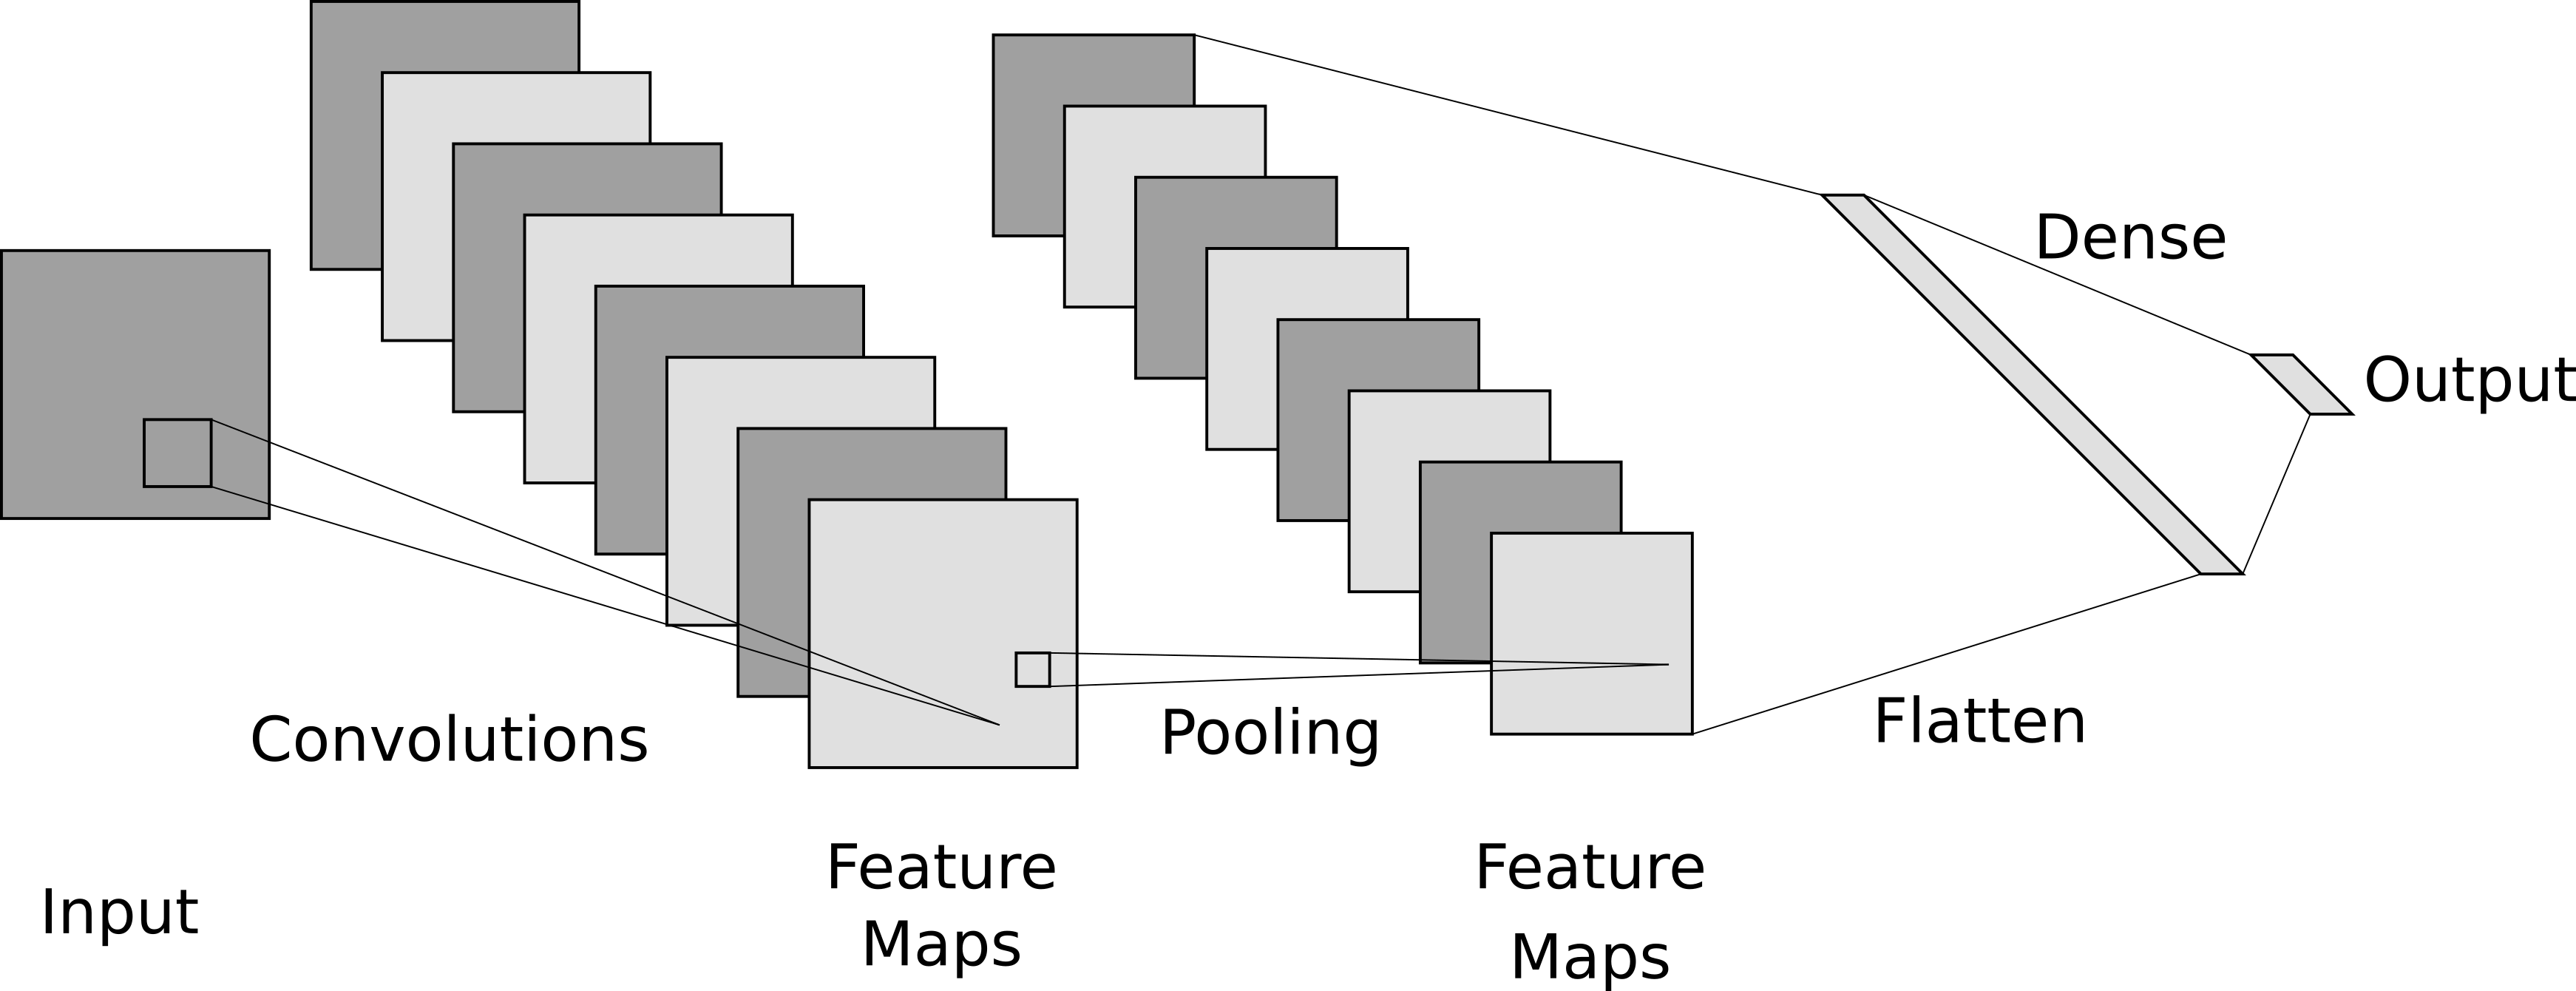
\includegraphics[width = \textwidth]{figures/cnn_layer.png}

	\caption
	[A graphical representation of a convolutional neural network.]
	{ A graphical representation of a convolutional neural network. Figure
	generated with \cite{cnn_diagrams}.}

	\label{fig:cnn_layer}

\end{figure}

\subsection{Residual Neural Networks}
Adding more layers to a neural network usually improves the performance, the
popular intuition for this is that with each subsequent layer the network is
able to learn more complex features of the image with which to make it's
classification. In fact adding more layer should never decrease the 
performance of a network, because the new layers could be set to be the 
identity, which would result in the same output from the network. However, it 
has been demonstrated that adding too many layers to a simple neural network 
will reduce performance, suggesting that the optimisation of
larger networks leads to degradation\cite{He_2016_CVPR}.

One method which has been shown to counter the degradation of deep networks, 
is the use of residual neural networks (ResNet). In a ResNet, the input to 
each layer is combined with the results of the convolutions as part of the 
input to a future layer; in effect, the identity transformation has been added
to the set of filters in the layer. An example of these shortcut connections 
is shown in Figure \ref{fig:short_connect}\cite{He_2016_CVPR}. 

\begin{figure}

	\centering

	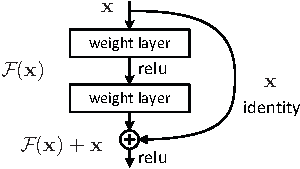
\includegraphics[width = 0.6\textwidth]{figures/short_connect.pdf}

	\caption
	[An example of a shortcut connection in a convolutional neural network.]
	{ An example of a shortcut connection in a convolutional neural network.
	Figure from \cite{He_2016_CVPR}.}

	\label{fig:short_connect}

\end{figure}

\section{Supervised Learning}
Supervised learning is the process of teaching a neural network to accurately
predict the correct output, the ground truth, for a given input. The network is 
optimised by minimising the loss function, which quantifies the difference 
between the network output and the ground truth. The choice of loss function 
is dependent on the problem being considered, specific examples will discussed 
in subsequent chapters, which will detail the CNN algorithms developed as part 
of this thesis.

The output of a neural network, g(x), is the result of a chain of function 
evaluations and matrix multiplication; for a network with $n$ layers,
\begin{equation}
	g(x) = f^n(W^n f^{n-1}(W^{n-1} \;...\; f^1(W^1 x) \;...\; ).
\end{equation}
where $g$ is the output of the network, $x$ is the input, $f$ are the 
activation functions for each layer, and $W$ are the weights for each layer. 
The loss of the network is given by the loss function, L,  evaluated on the 
output of the network and the ground truth, y,
\begin{equation}
	L(y, g(x)).
\end{equation}

To make accurate predictions with a NN, quantified by the loss function, the
weights and biases of the network need to be optimised. The backpropagation
algorithm\cite{Rumelhart1986} is currently the most widely used algorithm for
minimising the loss function by adjusting the weights and biases in the network.

Consider the weights for the $j^{th}$ node in the $i^{th}$ layer of a network,
$W^{ij}$, the loss function varies with respect to these weights as $\partial 
L/\partial W^{ ij }$, by adjusting the weights according to this gradient we 
can minimise $L$. If we adjust the weights with,
\begin{equation}
	\Delta W^{ ij } = -\eta \frac{\partial L}{\partial W^{ ij }},
\end{equation}
for positive learning rates, $\eta > 0$, we are guaranteed to reduce the loss. 
The backpropagation algorithm provides an algorithm for calculating the 
derivatives required to adjust the weights in each layer.

TODO>>>>>>>

% To calculate the derivative in Equation \ref{eq:weight_change}, we start with
% the chain rule,
% \begin{equation}
% 	\frac{\partial L}{\partial W^{ ij }} = \frac{\partial L}{\partial a^j}
% 	\frac{\partial a^j}{\partial W^{ ij }},
% \end{equation}
% where $a^j$ is the activation function. The activation function can be written
% in terms of the weights, $w$, and the output of the $i^th$ layer
% \begin{equation}
% 	a^j = w^{ij} x^j
% \end{equation}

% where $a^i$ is the activation function for the $i^{th}$ layer. The first term is
% usually called the error, 
% \begin{equation}
% 	\delta^i = \frac{\partial L}{\partial a^i},
% \end{equation}
% this term will be discussed later. The second term can be calculated from the
% equation for the activation function for the $i^th$ layer,
% \begin{equation}
% 	\frac{\partial a^i}{\partial W^i} = \frac{\partial}{\partial W^i} \left( W^i \cdot x^{i-1}
% 	\right) = x^{i-1},
% \end{equation}
% where $x^{i-1}$ is the output from the previous layer of the network.

%The gradient of the loss with respect to the losses in the $i^{th}$ layer of the
%network is therefore,
%\begin{equation}
%	\frac{\partial L}{\partial W^i} = \delta^i \; x^{i-1},
%\end{equation}
%which defines a recursive relationship between the output of one layer and the
%gradient of the next. 

% The error, $\delta$, also follows a recursive relationship.
% \begin{align}
% 	\nonumber \delta^i &= \frac{\partial L}{\partial a^i}\\ 
% 	\nonumber &= \frac{\partial L}{\partial a^{i+1}} \; \frac{\partial a^{i+1}}{\partial
% 	a^i} \\
% 	\nonumber &= \delta^{i+1} \; \frac{\partial a^{i+1}}{\partial a^i} \\
% \end{align}
% Recalling that, 
% \begin{equation}
% 	a^{i+1} = W^{i+1} \; f(a^i),
% \end{equation}
% the error becomes,
% \begin{equation}
% 	\delta^i = f^\prime(a^i) W^{i+1} \delta^{i+1}.
% \end{equation}
% Therefore, the partial derivative of the loss function with respect to the
% weights in the $i^{th}$ layer is,
% \begin{equation}
% 	\frac{\partial L}{\partial W^i} = \left( f^\prime(x^i) W^{i+1} \delta^{i+1} \right) \cdot x^{i-1}
% \end{equation}

\subsubsection{Batch Normalisation}

\subsection{Regularisation}
\cite{Srivastava2014DropoutAS}
\cite{OrrGenevieveB.1998NNTo}
